%&pdflatex

\documentclass[12pt]{report}

\usepackage{algorithm}
\usepackage{algpseudocode}
\usepackage{amsmath} % for implementation of the matrix environment
\usepackage{blindtext}
\usepackage{caption}
\usepackage{color}
\usepackage[pdftex]{graphicx} \graphicspath{{./plots/}}
\usepackage{epstopdf} \epstopdfsetup{update} % only regenerate pdf files when eps file is newer
\usepackage{float} % figure groups aka floats
\usepackage{forest} % for MFS elimination tree diagram
\usepackage[left=3.5cm, right=2.5cm]{geometry} % margins
\usepackage[hidelinks]{hyperref} % ToC/LoA/LoF/LoT entries are links
\usepackage{mathptmx} % Times New Roman like font
\usepackage{pdfpages} % for inserting pdf as the initial pages
\usepackage{setspace} \onehalfspacing % 1.5 line spacing
\usepackage{subcaption}
\usepackage{xfrac} % nice slanted fractions
\usepackage{minted} % for code listings

\captionsetup[figure]{labelfont={bf}, textfont={small}}
\captionsetup[subfigure]{labelfont={bf}, textfont={small}}

\newcommand{\bt}{\blindtext}
\newcommand{\eps}{\varepsilon}
%\newcommand{\rev}[1]{\textcolor{red}{#1}}
\newcommand{\rev}[1]{#1}
\newcommand{\T}[1]{\texttt{#1}}
\newcommand{\myparagraph}[1]{\paragraph{#1}\mbox{}\\} % adds newline after paragraph
\newcommand{\source}[1]{Source: {#1} } % for source in figures

\algnewcommand\And{\,\textbf{and}\,}
\algnewcommand\Or{\,\textbf{or}\,}
\algnewcommand{\LineComment}[1]{\State \(\triangleright\) #1}


\begin{document}


\includepdf[pages={-,{}}]{initial-pages.pdf} % `-' for all pages, `{}' for an empty page

\tableofcontents


\chapter{Preface}

% todo: if problem statement is moved, there should be some topic clarification here...
\section{Problem statement}
Purpose of this study is to compare performance of:
\begin{itemize}
    \item low-level, MPI-based implementation of graph algorithm
    \item high-level solution, developed in Spark-GraphX
\end{itemize}
Important points:
\begin{itemize}
    \item my target are supercomputer environments (as compared to e.g. commodity clusters, which Hadoop-derived solutions, Spark being among them, seem to be designed for)
    % todo: why important? homogenous hardware, fast interconnects, shared filesystem offering high-performance
    \item whole graph is available at launch, on shared filesystem
    \item graph is static and no modifications at runtime are permitted (although graph elements might be moved between nodes for load-balancing purposes)
\end{itemize}

\section{Motivation}
A couple of factors influenced decision to pick this topic. Most important of them are described below.

\subsection{Why graph algorithms?}
Graphs are very flexible structures, which can be used to model wide-array of very challenging problems. For example:
\begin{itemize}
    \item web graph - analyze links that interconnect web documents to asses their importance or thematic similarity in order to improve search results
    \item social graph - represents relationships between peoples' online avatars, and thus can help find groups with shared characteristics (beliefs, interests, preferences) which could be used for content targeting, be it news, ads or products in online shop 
    \item knowledge graph - try to express relationships between concepts to aid AI algorithms in quest for true intelligence
    \item real-life networks (power grid, computer, telecommunication, oil delivery, roads) - many crucial pieces of infrastructure form graph-like structures, therefore any analysis or simulation involving them turns into graph problem
\end{itemize}

\subsection{Why parallel?}
Some of the graphs that are already being analyzed are too large for a single machine. And these are just information about structure of graph - what about situations where each vertex and edge come with significant amount of metadata? Examples listed below should give reader some idea about order of magnitude of the problem:
\begin{itemize}
    \item Friendster Social Graph - $65,6 \times 10^6$ nodes, $1,8 \times 10^9$ edges (website has been shut down in 2015)
    \item Facebook Social Graph - no data available, but at the beginning of 2018 Facebook reported to have nearly $ 2.2 \times 10^9 $ of active users. If vertex-to-edges ratio is similar to that of Friendster (around 1-to-27), amount of edges could be greater than $50 \times 10^9$ \cite{facebook-user-count}
    \item Web Data Commons - graph of hyperlinks, probably the largest openly available such graph outside of companies like Google, Yahoo! or Microsoft. It contains $3.5 \times 10^9$ webpages and $ 128 \times 10^9 $ of hyperlinks. \cite{wdc-graph}
\end{itemize}
More examples of real-life graphs can be found here \cite{gap-graphs}.

\subsection{Why low-level implementation?}
The problem of huge graphs has not gone unnoticed and multiple solutions has been developed, usually in the form of fairly complex graph processing engines. They make writing algorithms for large-scale graph processing easier by handling a lot of stuff transparently (like scheduling, auto-scaling, fault tolerance, support for disk spilling, interacting with different storage mediums). But it does not come for free, as suggested in \cite{mcsherry-scalable-overhead}. It would be interesting to see exactly how much overhead is being introduced.



\section{Related efforts}
% @todo: shared memory & distributed memory

\subsection{Benchmarks}
One could expect to find benchmarks for both parallel algorithms and machines/clusters, but only the second ones seem to be available. Their purpose is to assess how well infrastructure is suited to running graph algorithms.

\subsubsection{Graph500}
Graph500 \cite{www-graph500} is a graph-oriented equivalent of Top500 list. It provides reference problems, which are used to rank supercomputers (currently, there is BFS and SSSP). Graph500 provides reference implementation, but benchmarkers can use their own, provided in conforms to problem specification.

\begin{figure}
    \centering
    
    \begin{subfigure}[h]{1.0\textwidth}
        \centering
        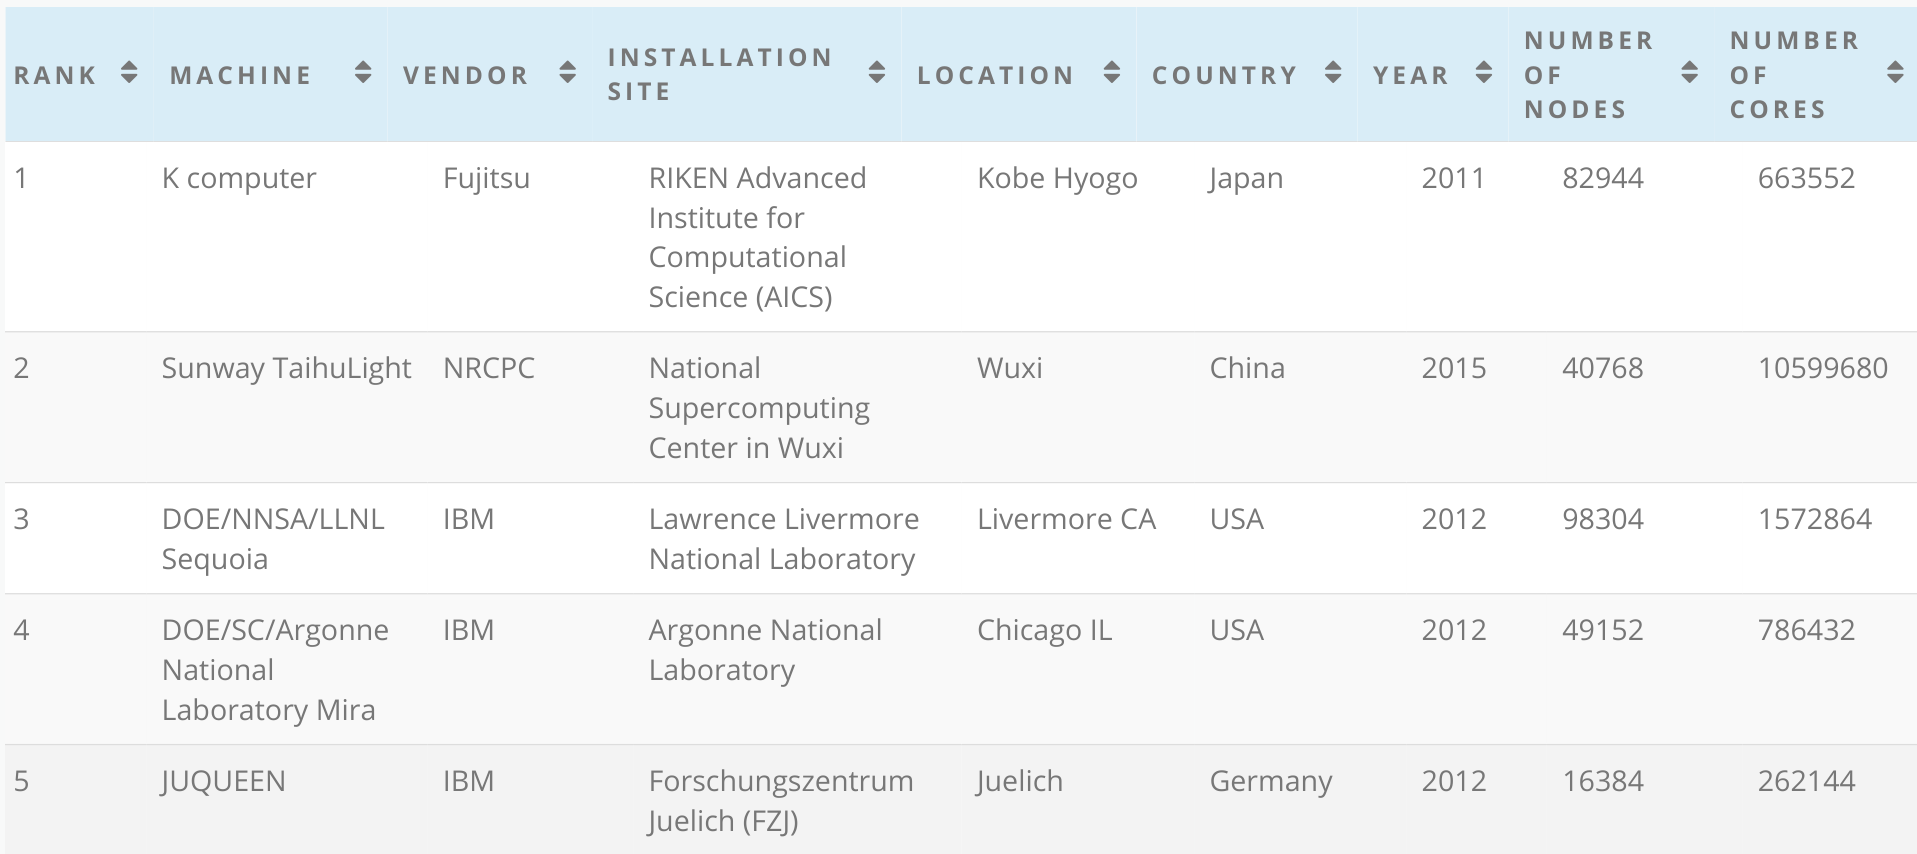
\includegraphics[scale=0.2]{images/graph500-bfs.jpg}
        \caption{BFS}
        \label{fig:graph500-bfs}
    \end{subfigure}
    
    \begin{subfigure}[h]{1.0\textwidth}
        \centering
        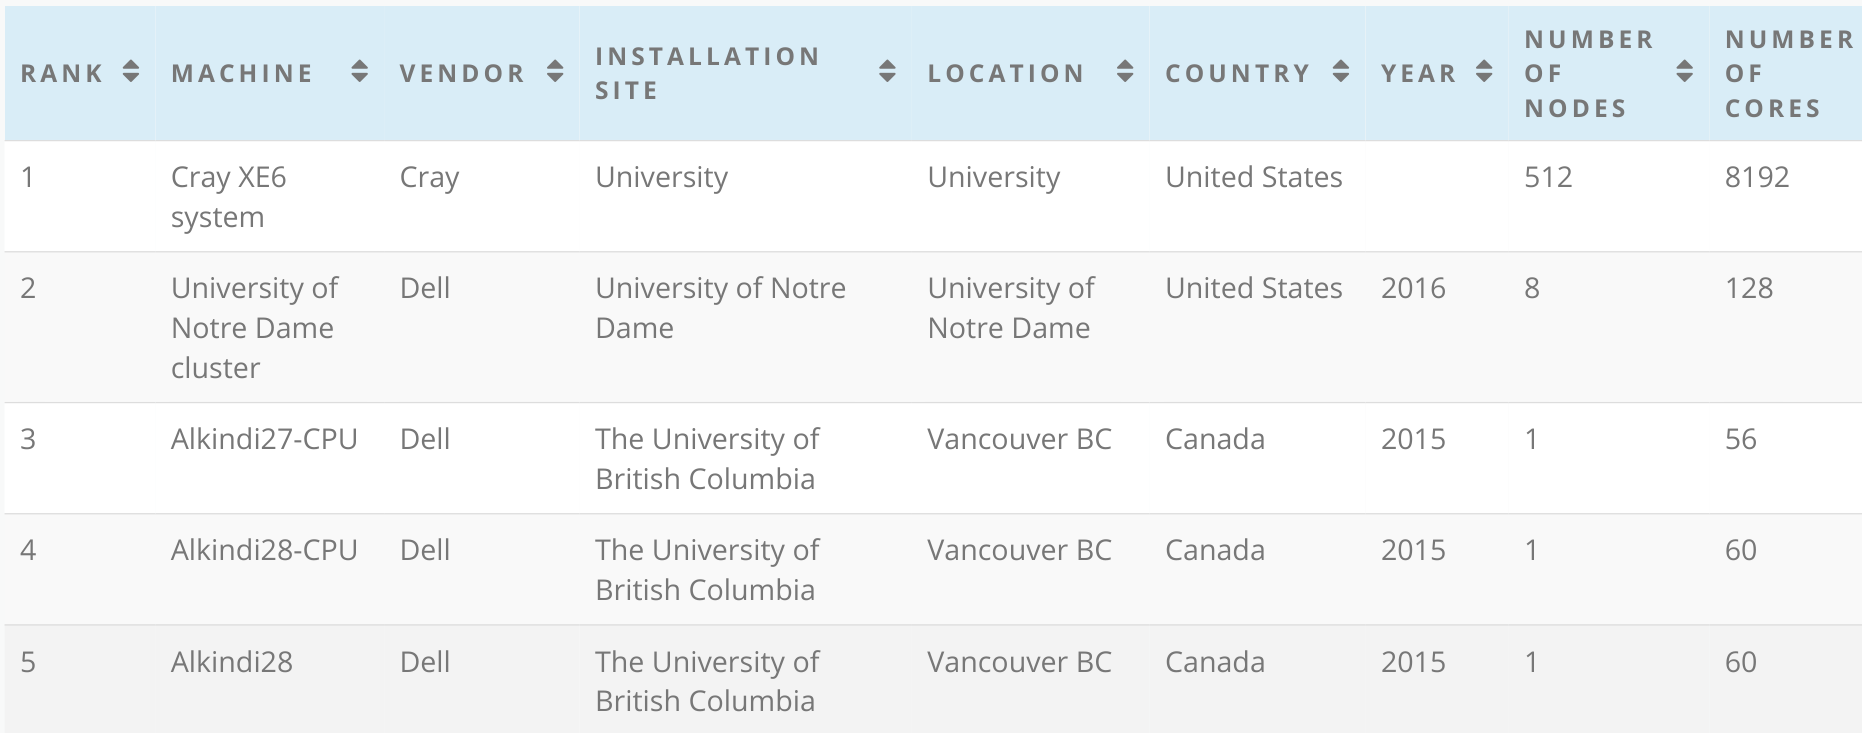
\includegraphics[scale=0.2]{images/graph500-sssp.jpg}
        \caption{SSSP}
        \label{fig:graph500-sssp}
    \end{subfigure}
    
    \caption{Five highest-ranked supercomputers on Graph500 list (Nov 2017), for two problems: BFS and SSSP}
    \source{\cite{www-graph500}}
\end{figure}

\subsubsection{The GAP Benchmark Suite}
The GAP Benchmark \cite{gap-graphs} is suite of benchmarks (specification + implementation) geared towards evaluating performance of shared memory system in context of graph computations. It is consisted of 6 kernels: Breadth-First Search (BFS), Single-Source Shortest Paths (SSSP), PageRank (PR), Connected Components (CC), Betweenness Centrality (BC), Triangle Counting (TC).

\subsection{Frameworks}
% todo: divide frameworks into those two groups
% todo: argumentation against distributed from GraphChi paper
Feature-rich platforms which aim to simplify solution development by introducing higher-level abstractions. They can be divided into two groups:
\begin{enumerate}
    \item Single-node - despite being limited to single node, they can process large graphs by loading only parts of them into memory for processing. Some examples:
    \begin{itemize}
        \item GraphChi
        \item X-Stream
    \end{itemize}
    
    \item Distributed - designed to work with graphs partitioned across multiple nodes. They may or might not support spilling to disk if allocated memory is insufficient. In this group we have:
    \begin{itemize}
        \item Apache Giraph
        \item Apache GraphX
        \item Microsoft Graph Engine
    \end{itemize}
\end{enumerate}

\subsubsection{GraphChi}
GraphChi is a disk-based system for computing efficiently on graphs with billions of edges.

\begin{itemize}
    \item Computational model is similar to Pregel (\textit{update} function executed for each vertex over and over again), with one significant difference - \textit{update} function is not guaranteed to observe values from previous ''super-step``, some of them can see updates from current one.
    \item The core part of GraphChi is \textit{Parallel Sliding Windows} algorithm (explained below)
\item before graph can be loaded into GraphChi it must be preprocessed
\item GraphChi can also support evolving graphs (but certain modificaions are required to PSW algorithm)
\end{itemize}


\myparagraph{Parallel Sliding Window}
PSW processes graphs in three stages:
\begin{enumerate}
    \item load a subgraph from disk
    \item update the vertices
    \item write updates values to disk
\end{enumerate}

\\
Step 1: Loading
\\
Vertices are split into intervals, each interval has shard associated. Shard contains all edges that have destination in given interval, sorted by source. Intervals are chosen to balance numer of edges in each shard. Their number is such that any shard can be loaded to memory.

\noindent
Processing is done interval after interval. For each interval, corresponding shard (called memory-shard) is loaded (all in-edges). Then out-edges are loaded from other shards (in theory, shard can contain some out-edge). Because edges are sorted by source and intervals are sorted by vertex id, out-edges for given interval in any shard should be stored consecutively.
Therefore, for each interval we need to read at most $P-1$ blocks (where P is number of intervals).

\begin{figure}
    \centering
    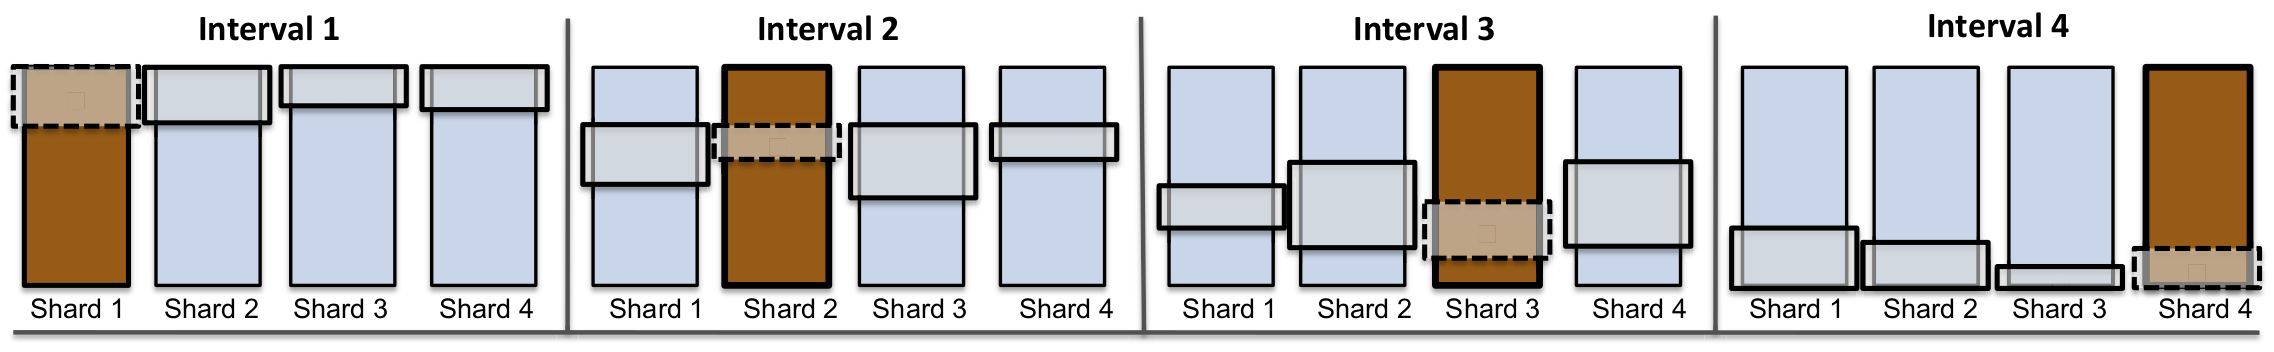
\includegraphics[scale=0.2]{images/graphchi-sliding-window.jpg}
    \caption{Visualization of the stages of one iteration of PSW. In-edges for current interval are read from corresponding shard (in dark color) while out-edges are read in blocks from all other shards}
    \label{fig:graphchi-psw}
    \source{\cite{graphchi-paper}}
\end{figure}

\\
Step 2: Updating
\\
After loading interval from disk, user-defined \textit{update} function is executed for each vertex in parallel. If vertices have neighbours in the same interval, race conditions might occur. This is solved by marking those vertices as critical and updating them in sequential order.

\\
Step 3: Writing updates to disk
\\
After all vertices are processed, changes must be written to disk so that they are available to subsequent computations. Contents of memory-shard are rewritten completely, updating other shards is done by writing whole blocks (which were loaded into memory in step 1).

%

stores graph both in CSR and CSC (in-edges)
implements asynchronous model (uses most recent values of edges and vertices)
generic solutions, such as systems that extend main memory by using SSDs, do not perform well

% todo: METIS [25], requires hundreds of gigabytes of memory to work with graphs of billions of edges.
% todo: can store web-graphs in only 4 bits/edge (see [8, 12, 17, 23]).

\subsubsection{X-Stream}
X-Stream \cite{xstream-paper} builds on the ideas proposed by GraphChi.

X-Stream in order to improve performance, uses slightly different computational paradigm than the one proposed by Pregel (and copied by many successful frameworks). Instead of \textit{update} function, X-Stream requires pair of function: \textit{edge-scatter} and \textit{edge-gather}. The fact that there are two functions instead of one is far less significant than edge-centeredness of this approach: 
\begin{itemize}
    \item edge-centric scatter takes as input an edge, and computes, based on the data field of its source vertex, whether an update value needs to be sent to its destination vertex
    \item edge-centric gather takes as input an update, and uses its value to recompute the data field of its destination vertex
\end{itemize}

Graph is divided into \textit{streaming partitions}. Each partitions contains:
\begin{itemize}
    \item vertices
    \item corresponding edges (out-edges)
    \item all updates produced by scatter-gather functions for edges with destination vertex in partition
\end{itemize}
First two sections remain unchanged for the duration of the algorithm. Update list is recomuted every gather phase.

The overall computation is structured as a loop, terminating when some application-specific criterion is met. Each loop iteration consists of scatter phase and gather phase. For gather phase to start, scatter phase must be executed on all edges. Hence, X-Stream scatter-gather is synchronous. %todo: shuffle!

Since edges are stored in partition with their edge sources and computed updates with destination, they must be redistributed (\textit{shuffling}).

By adopting edge-centric computational model and tailored on-disk representation, X-Stream relies solely on sequential access to storage, improving processing performance.

\subsubsection{Apache Giraph}
Written in Java, Apache Giraph is open-source implementation of model popularized by Google, often referred to as \textit{Pregel-model}. The name comes from Google's own graph processing system, which has been described in \cite{google-pregel}. Unfortunately, Pregel itself is not available to wider public in either source or binary version.

\noindent
Apache Giraph to work requires Hadoop cluster. It can use MapReduce or run directly on YARN.

\noindent
As in Bulk Synchronous Parallel model, computations in Giraph are performed in supersteps. In each superstep each active vertex invokes the \textit{Compute} method provided by the user. The \textit{Compute} method receives messages sent to the vertex in the previous superstep. It can also access values associated with current vertex and all its outgoing edges. Based on received messages and available values, it can:
\begin{itemize}
    \item modify those values (for vertex or outgoing edges) - no access to other vertices and edges
    \item send messages to other vertices - messages can be sent to any vertex, not only immediate neighbours
\end{itemize}
Model also allows mutations to graph by removing vertices or edges.

\noindent
Consecutive supersteps are separated by barriers:
\begin{itemize}
    \item messages sent during superstep N are delivered in superstep N+1
    \item vertices start computing superstep N+1 only after all vertices finished computation of superstep N
\end{itemize}

Any vertex can declare that it does not want to be active anymore. However, any incoming message will make the vertex active again. The computation halts after the vertices have voted to halt and there are no messages in flight.

% use https://codebeautify.org/javaviewer to fix indendation
\begin{figure}
    \centering
    \begin{minted}{java}
    public void compute(Iterable<DoubleWritable> messages) {
        double minDist = Double.MAX_VALUE;
        for (DoubleWritable message : messages) {
            minDist = Math.min(minDist, message.get());
        }
        if (minDist < getValue().get()) {
            setValue(new DoubleWritable(minDist));
            for (Edge<LongWritable, FloatWritable> edge : getEdges()) {
                double distance = minDist + edge.getValue().get();
                sendMessage(edge.getTargetVertexId(), new DoubleWritable(distance));
            }
        }
        voteToHalt();
    }
    \end{minted}
    \caption{Sample \textit{Compute} method which can be used for SSSP calculation}
    \label{fig:giraph-code-sample}
    \source{\cite{giraph-intro}}
\end{figure}

Apache Giraph automatically performs checkpoints based on configurable interval (expressed in supersteps). Checkpoint is performed by saving current state of the graph to HDFS. In case of failure, Giraph should automatically recover, provided correct checkpoint is available. \cite{giraph-book}

% todo: partitioning, Giraph++ as possible solution

\noindent
At the time of writing, the most recent version of Apache Giraph is 1.2.0. Documentation can be found in \cite{giraph-intro}

\subsubsection{GraphX}
GraphX is a graph processing library for Spark. Therefore, knowledge of Spark is required to understand GraphX.

\myparagraph{Spark}
Apache Spark is a general-purpose cluster computing system with high-level APIs in Java, Scala, Python and R. It is written mostly in Scala, which means it requires JVM to run. Unlike Apache Giraph, Spark does not require Hadoop installation to work, it can be deployed as standalone cluster (but it can work on top of YARN if necessary).

\noindent
RDD (\textit{Resilient Distributed Dataset}) is most basic computational abstraction in Spark. It can be thought of as list of tuples, on which we can perform transformations using higher-order functions (\textit{map}, \textit{filter}, \textit{reduce}, \textit{sort} etc.) and operators more common in world of SQL databases (\textit{groupby}, \textit{join}). Every transformation yields new RDD (at least conceptually).
\begin{itemize}
    \item \textit{distributed} - RDDs are partitioned across all processes
    \item \textit{resilient} - Spark remembers how each partition has been created. In case of process failure partition can be transparently recreated.
\end{itemize}

\noindent
Operations on RDDs are lazily evaluated - Spark doe not execute anything until we request results. When such an operation is issued, Spark:
\begin{itemize}
\item groups operations into stages. Ideally, computations should form single stage - this would be most efficient and can be achieved if our computations do not require repartitioning of RDD (\textit{shuffle}). Each shuffle equals stage split.
    \item for each stage tasks are generated - one task for each part of the RDD within given stage. Tasks within stages contain same computations, but are executed on different partitions.
    \item tasks are sent to processes which are responsible for given partition (computations are sent to data)
\end{itemize}
Spark transparently serializes functions we pass to RDD transformations.

\noindent
RDD transformations are unable to share data across partitions (or even across data units within partition). Therefore, Spark introduces two types of shared variables:
\begin{itemize}
    \item \textit{broadcast variables} - read-only variables accessible to all nodes. This is more of a performance optimization that extension of programming model and comes in handy when we shuffle a lot
    \item \textit{accumulators variables} - variables that can be only "added" to through an associative and commutative operations
\end{itemize}

\noindent
When it comes to IO using Spark, out-of-the-box Spark can read from and write to files (either ordinary files, possibly stored on shared storage, or HDFS files). There are numerous third party connectors available which enable parallel operations against databases, message queues and so on.

\noindent
Most recent version of Spark available at the time of writing was 2.3.0. Documentation can be found in \cite{spark-doc}.

\myparagraph{Back to GraphX}
% cite in paragraph
\begin{figure}
    \centering
    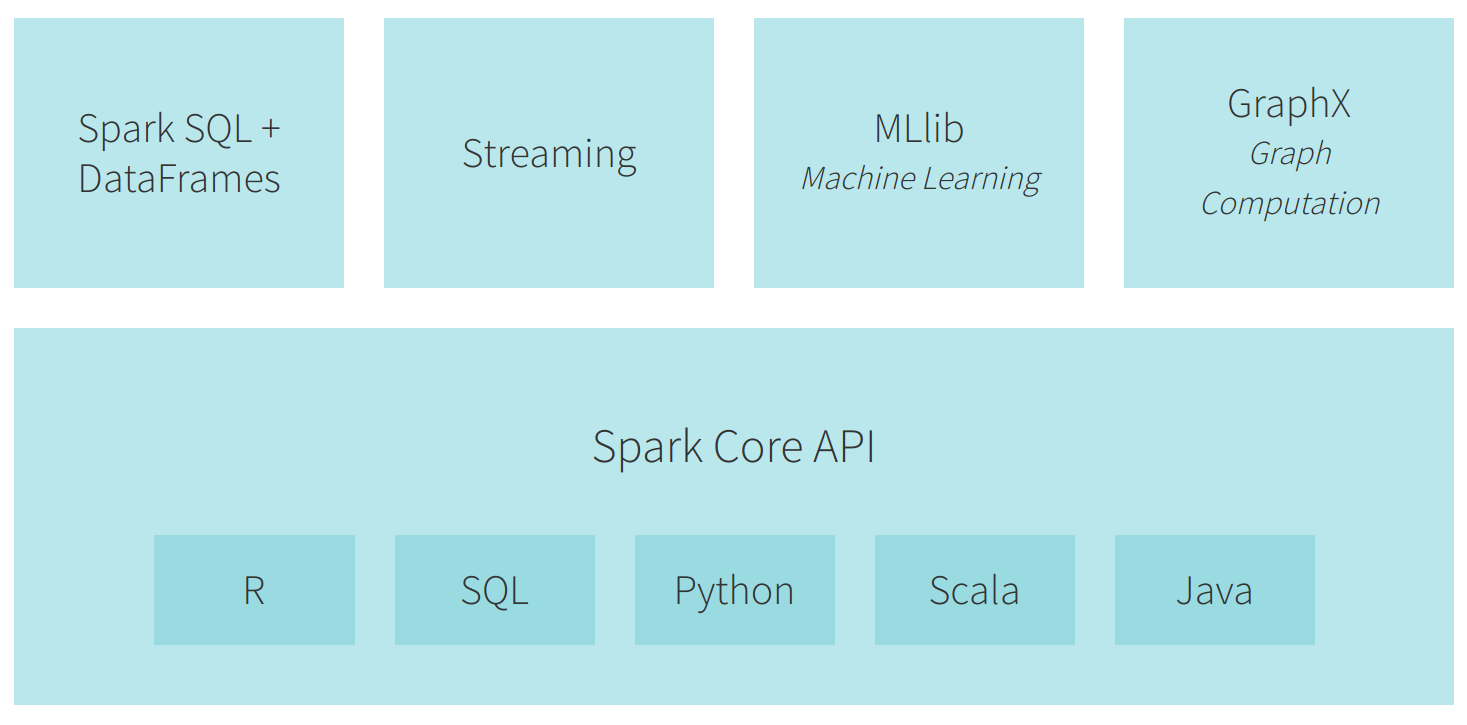
\includegraphics[scale=0.2]{images/spark-ecosystem.jpg}
    \caption{Spark ecosystem - relationship between Spark and GraphX}
    \label{fig:spark-ecosystem}
    \source{\cite{databrics-spark-ecosystem}}
\end{figure}

At a high level, GraphX extends the Spark RDD by introducing a new Graph abstraction: a directed multigraph with properties attached to each vertex and edge (often referred to as \textit{Property Graph}). To support graph computation, GraphX exposes a set of fundamental operators (e.g., subgraph, joinVertices, and aggregateMessages) as well as an optimized variant of the Pregel API. In addition, GraphX includes a growing collection of graph algorithms and graph builders to simplify graph analytics tasks. User can also specify custom partitioning, best suited to problem being solved.

\noindent
Since GraphX's Graphs are built on top of Spark RDDs, they inherit their properties: immutability, distribution and fault-tolerance. To avoid excessive overhead involved in pure immutability, GraphX uses some variant of copy-on-write scheme. 

\noindent
Fundamental operators include:
\begin{itemize}
    \item \textit{VertexRDD}, \textit{EdgeRDD}, \textit{EdgeTripletRDD} (edge + both vertices it connects) supporting most of the standard RDD operations
    \item graph statistics: vertex/edge count, vertex degrees
    \item reversing, subgraphing, masking
    \item groupping edges, joining vertices
    \item accessing neighbours
    \item messaging - takes two functors, \textit{sendMsg} which is applied to each triplet in order to produce message (iterates over all edges) and \textit{mergeMsg} used to merge messages sent to each vertex. It produces VertexRDD of merged messages.
\end{itemize}

\noindent
Algorithms implemented:
\begin{itemize}
    \item page rank
    \item connected components
    \item triangle counting
    \item strongly connected components
\end{itemize}

\noindent
Pregel-like API exposed by GraphX is slightly different from what Giraph offers. We pass three functors:
\begin{itemize}
    \item \textit{vprog} - vertex program, processes received messages
    \item \textit{sendMsg} - invoked on all out-edges, used to compute optional message to destination vertex
    \item \textit{mergeMsg} - merges messages destined to the same vertex
\end{itemize}
Unlike in Giraph, messages can be only sent to neighbouring vertices.
Vertices that do not receive any message are skipped. Operation terminates when there are no messages remaining (or iteration limit has been reached).

% Graph loaders
\noindent
Graphs can be created from:
\begin{itemize}
    \item text files containing edge list
    \item RDD of edges (plus, optionally, RDD of vertices)
\end{itemize}

% todo: partitioning (during loading and repartitioning later on)

\noindent
GraphX releases are synchronized with Spark's. Therefore, most recent version available at the time of writing was 2.3.0. Documentation can be found in \cite{graphx-doc}.

\subsubsection{Microsoft Graph Engine}
Microsoft Graph Engine is a new name for technology that began as Trinity graph engine \cite{trinity-engine}. It is written in C++/C\# and requires .NET to work (both Windows and Linux builds are supported).

\noindent
MGE has two major components:
\begin{itemize}
    \item RAM store - distributed, in-memory key-value store. Optionally supports WAL log for durability. Stores blobs to which we can give schema using TSL.
    \item declarative message passing engine
\end{itemize}
Both functionalities heavily rely on \textit{Trident Specification Language}. TSL is a kind of interface definition language, which is used to define schemas for RAM store cells, format of messages and protocols. Responsibility for providing code for encoding/decoding data structures and stubs for communication (that's why protocol specification are needed in IDL) is shifted from programmer to special Visual Studio plugin. Conceptually, the idea is very similar to CORBA IDL or Slice language for Internet Communications Engine.

After studying documentation \cite{mge-website} MGE seems more like a general-purpose computation engine rather than graph processing framework. Out-of-the-box it does not offer any Graph-related data structures or operations, but they can be built on top of it. This is how creators justify their design choices:

% todo: style this quote
\begin{quote}
``Due to the diversity of graphs and the diversity of graph applications, it is hard, if not entirely impossible, to support all kinds of graph computations using a fixed graph schema. Instead of using a fixed graph schema and fixed computation paradigms, Trinity allows users to define their own graph schemas, communication protocols through Trinity specification language (TSL) and realize their own computation paradigms.''
\end{quote}


% todo: turboGraph: outperforms GraphChi, but exploits properties of SSDs
% todo: study newer papers (those that cite GraphChi, X-Stream, ...
% todo: memory usage of those frameworks, how do they compare? (inmemory, spilling to disk, ...)
% Neo4J
% todo: performance comparison for those that can be done
% todo: performance results from papers
% spark: also based on key-value store, similar to Trinity?
% Picolo (spark-like)
% graphlab paper: graphlab: a new parallel framework for machine learning

% paper for partitioning: Community structure in large networks: Natural cluster sizes and the absence of large well-defined clus-
% R. Pearce, M. Gokhale, and N. Amato. Multithreaded Asynchronous Graph Traversal for In-Memory and Semi-External Memory.



\medskip


\chapter{Problem formulation} \label{chap:problem-formulation}

% introduce problems you'll be testing!

\section{Issues to be addressed in this work}

\subsection{(e.g.) Algorithmic challenges}

\subsection{(e.g.) Parallelization challenges}

\section{Functional requirements}

\begin{enumerate}
	\item Core functionalities
	\begin{enumerate}
		\item ...
		\item ...
		\item ...
	\end{enumerate}

	\item Adaptation strategies
	\begin{enumerate}
		\item ...
		\item ...
	\end{enumerate}

	\item Visualization and profiling
	\begin{enumerate}
		\item ...
		\item ...
		\item ...
		\item ...
	\end{enumerate}
\end{enumerate}


\section{Non-functional requirements}

\begin{enumerate}
	\item Performance and complexity
	\begin{enumerate}
		\item ...
		\item ...
		\item ...
	\end{enumerate}

	\item Development requirements
	\begin{enumerate}
		\item ...
		\item ...
	\end{enumerate}
\end{enumerate}


\chapter{Solution methodology} \label{chap:methodology}

\bt

\section{Method 1}

\bt

\section{Method 2}

\bt 

\section{Method 3}

Some nice matrices...

\begin{equation}
	A = \begin{bmatrix}
		1 &    &    &    &    &    &    & \\
		1 & -2 &  1 &    &    &    &    & \\
		  &  1 & -2 &  1 &    &    &    & \\
		  &    &  1 & -2 &  1 &    &    & \\
		  &    &    &  1 & -2 &  1 &    & \\
		  &    &    &    &  1 & -2 &  1 & \\
		  &    &    &    &    &    &  1 & \\
	\end{bmatrix}
	\hspace{1cm}
	B = \begin{bmatrix}
		0 \\
		4 \\
		4 \\
		4 \\
		4 \\
		4 \\
		0
	\end{bmatrix}
\end{equation}

Some nice diagrams...

\newcommand{\cv}[1]{ % column vector
	$\begin{bmatrix} #1 \end{bmatrix}$
}
\newcommand{\Cv}[1]{ { \cv{#1} } } % shortcut for tree leaves
\newcommand{\elim} { $\xrightarrow{E}$ }
\newcommand{\merge} { $\xrightarrow{M}$ }
\newcommand{\xtract} { $\xrightarrow{X}$ }

\begin{figure}[H]
	\centering
	\caption{Elimination tree for multifrontal solver}
	\label{fig:mfs-elim-tree}
	\begin{forest}
		for tree = {
			draw,
			edge={<-, line width=2pt},
			minimum height=2cm,
			anchor=north,
			align=center,
			child anchor=north
		},
		[ { \merge \cv{x_1 \\ x_5 \\ x_7} \elim \cv{x_1 \\ x_7 } }
			[ { \merge \cv{x_1 \\ x_3 \\ x_5} \elim \cv{x_1 \\ x_5} }
				[ { \merge \cv{x_1 \\ x_2 \\ x_3} \elim \cv{x_1 \\ x_3} }
					[ \Cv{x_1 \\ x_2} ]
					[ \Cv{x_2 \\ x_3} ]
				]
				[ { \merge \cv{x_3 \\ x_4 \\ x_5} \elim \cv{x_3 \\ x_5} }
					[ \Cv{x_3 \\ x_4} ]
					[ \Cv{x_4 \\ x_5} ]
				]
			]
			[ { \merge \cv{x_5 \\ x_6 \\ x_7} \elim \cv{x_5 \\ x_7} }
				[ \Cv{x_5 \\ x_6} ]
				[ \Cv{x_6 \\ x_7} ]
			]
		]
	\end{forest}
\end{figure}

\pagebreak

Some nice algorithms...

\newcommand{\U}{\mathcal{U}}

\begin{algorithm}
\caption{One iteration of the double-grid algorithm}
\label{alg:two-grid}

\begin{algorithmic}

	\State Compute the solution $\U^C$ on the coarse mesh
	\State Split each element of the coarse mesh, thus obtaining the fine mesh
	\State Compute the solution $\U^F$ on the fine mesh

	\For{\textbf{each} coarse mesh element $\eps_i$}
		\LineComment{$\rho_i$ is the relative error}
		\State $ \rho_i \gets \left|
				\frac {
					\U^F_i - \U^C_i
				} {
					\U^F_i
				}
			\right| $
	\EndFor

	\State $\rho_{max} \gets$ $max_i(\rho_i)$

	\For{\textbf{each} element $\eps_i$}
		\If {$ \rho_i > \tau \cdot \rho_{max} $}
			\State adapt the $\eps_i$ element (split into two halves)
		\EndIf
	\EndFor

\end{algorithmic}
\end{algorithm}

\pagebreak

Some nice figures...

\begin{figure}[H]
	\centering

	\caption[Double-grid h-adaptation strategy, steps 1-2] {
		Steps 1-5 of the double-grid h-adaptation strategy, quadratic B-splines
	}
	\label{fig:h-adapt-two-grid}

	\begin{subfigure}[h]{1.0\textwidth}
		\centering
		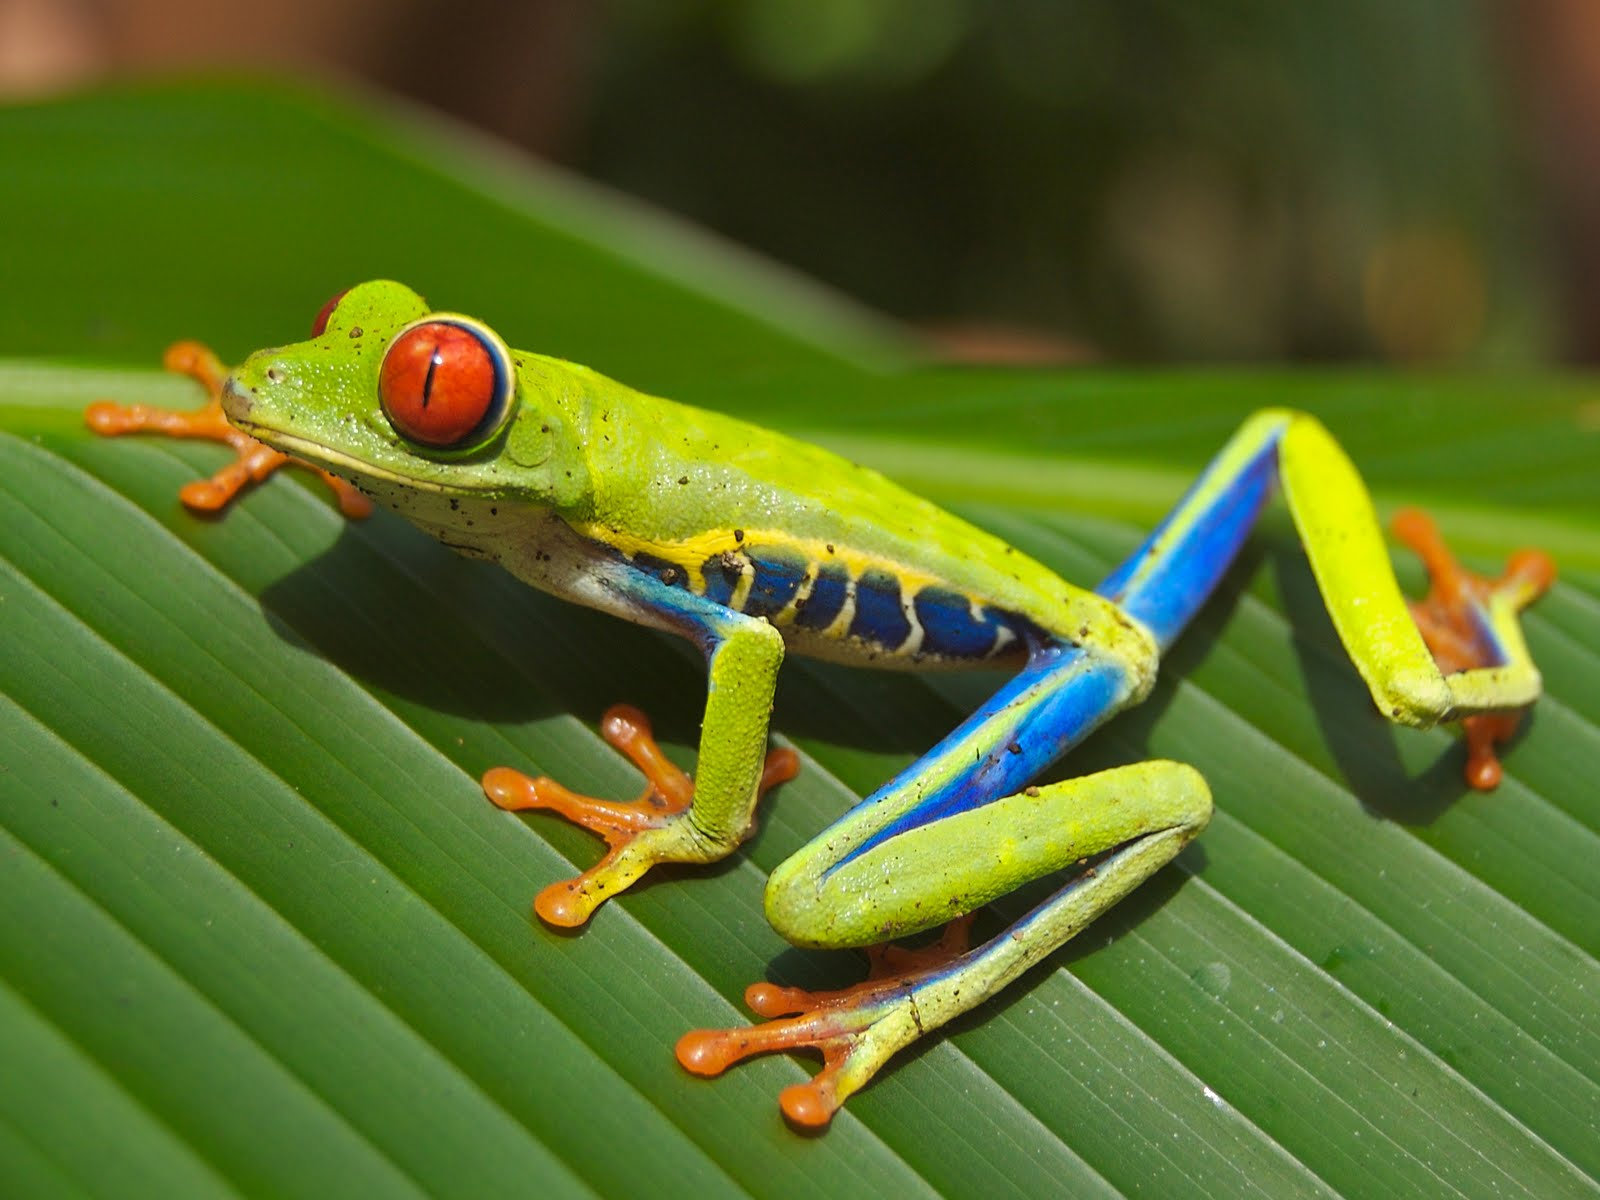
\includegraphics[scale=0.2]{frog.jpg}
		\caption{
			Step 1.
			A solution is delivered on coarse (4 elements) and fine grid (8 elements).
			Red line marks the coarse-grid solution, green line --- the fine-grid solution and black line --- the exact (analytic) solution.
		}
		\label{fig:h-adapt-two-grid-1}
	\end{subfigure}

	\begin{subfigure}[h]{1.0\textwidth}
		\centering
		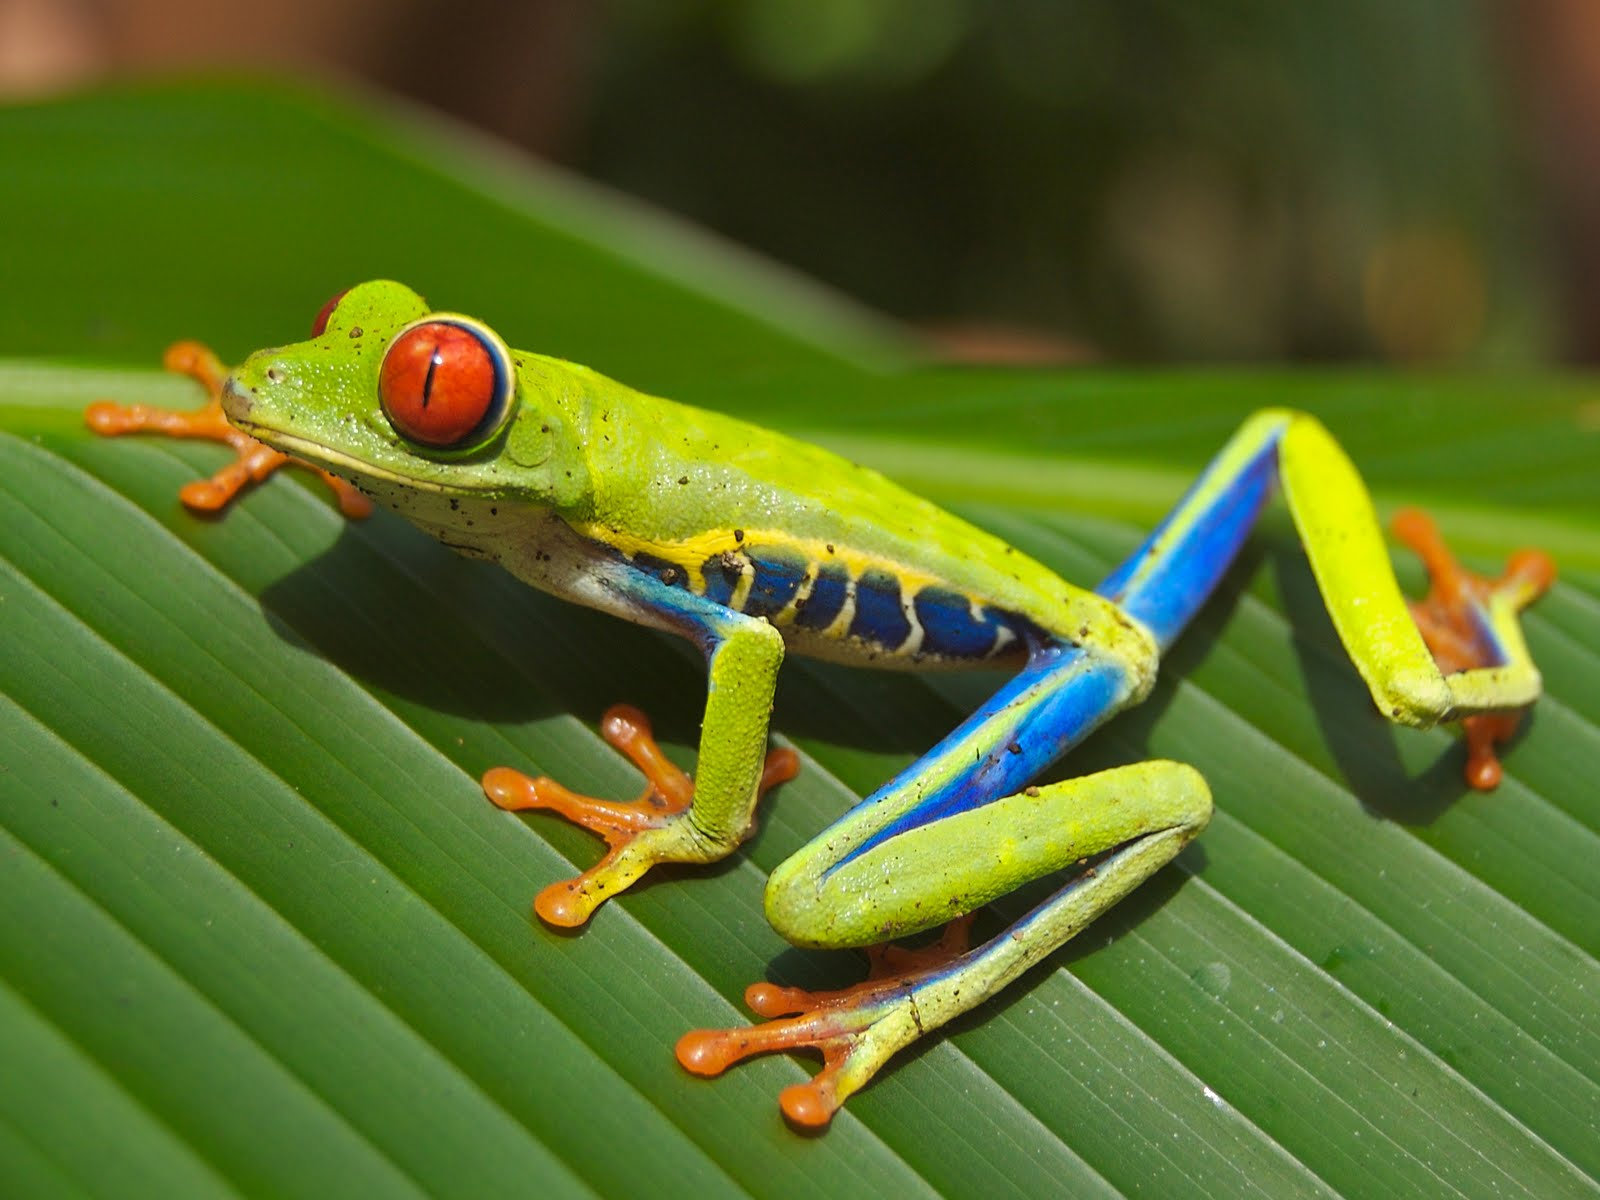
\includegraphics[scale=0.2]{frog.jpg}
		\caption{
			Step 2.
			Since the maximal error multiplied by $\tau$ (here set to 20\%) were lower than the error on any element,
			the algorithm halved all four elements after step 1.
		}
		\label{fig:h-adapt-two-grid-2}
	\end{subfigure}
\end{figure}


\begin{figure}[H]
	\ContinuedFloat % continue from previous page
	\caption[Double-grid h-adaptation strategy, steps 3-4]{} % for subcaption package to ensure proper numbering

	\begin{subfigure}[h]{1.0\textwidth}
		\centering
		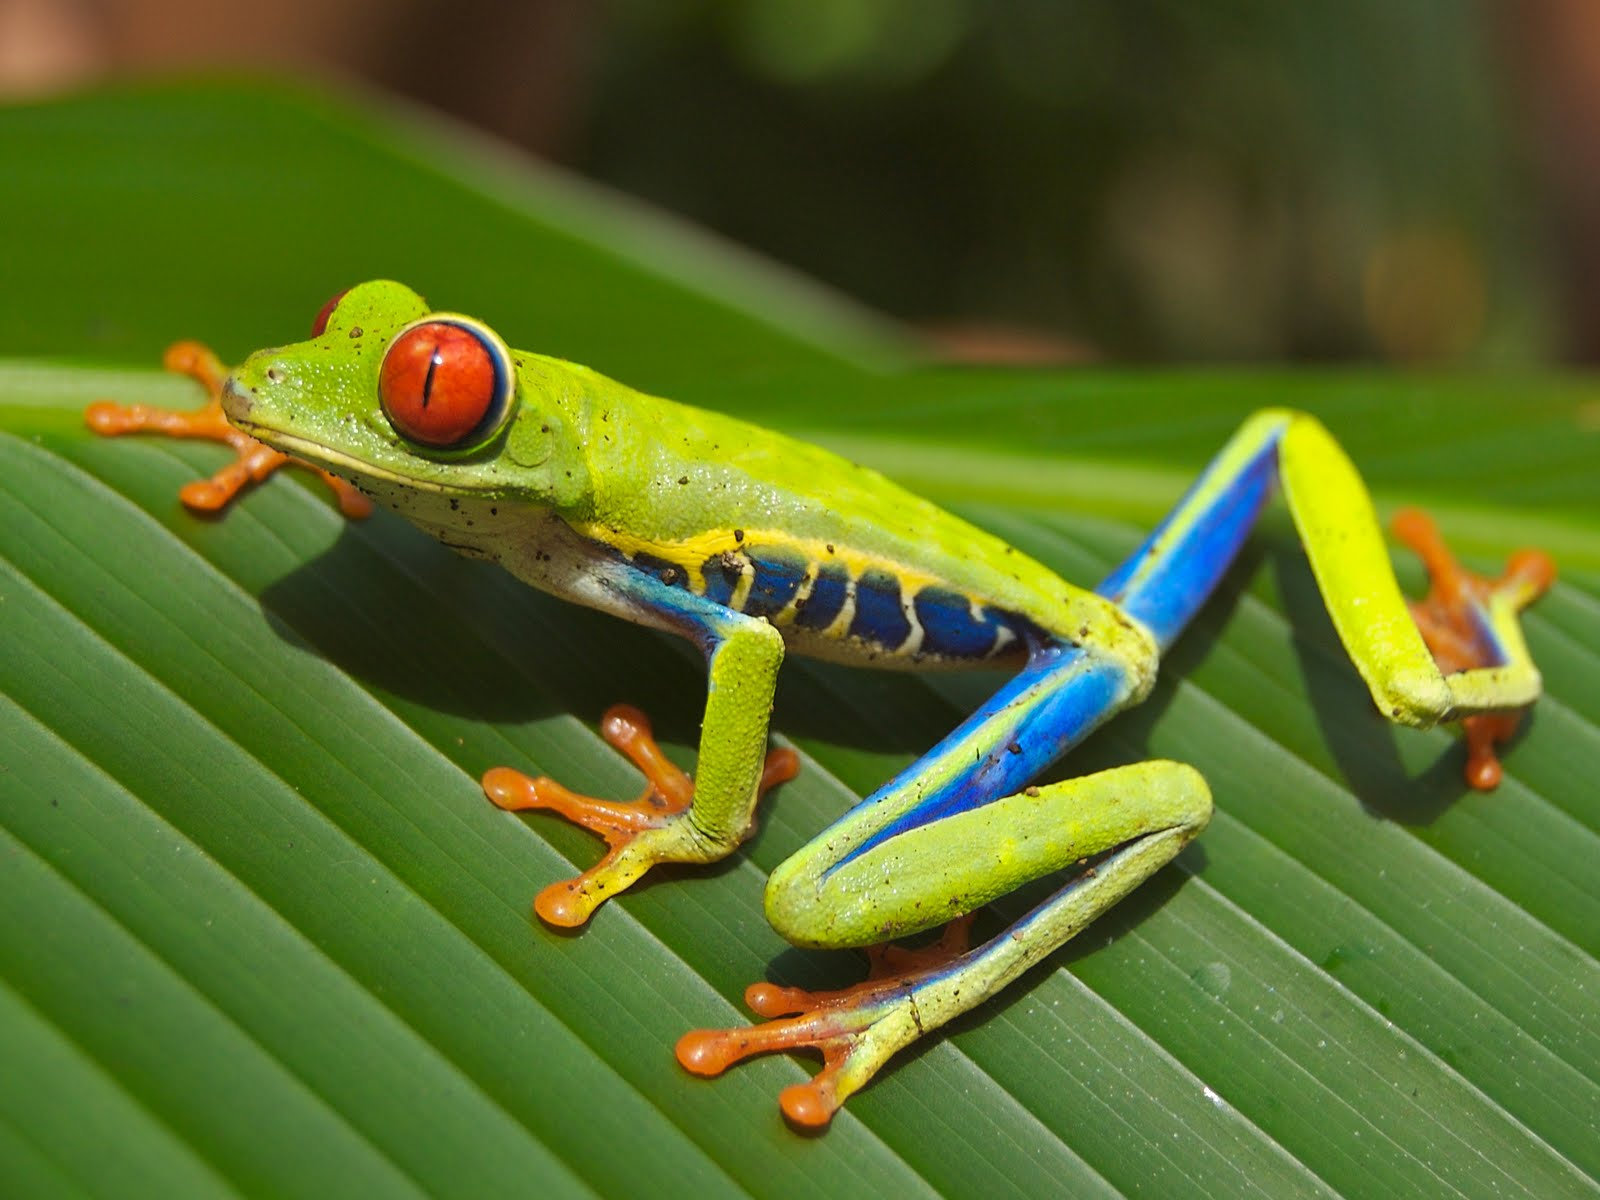
\includegraphics[scale=0.2]{frog.jpg}
		\caption{
			Step 3.
			The extreme left and right elements did not get refined after the step 2.
		}
		\label{fig:h-adapt-two-grid-3}
	\end{subfigure}

	\begin{subfigure}[h]{1.0\textwidth}
		\centering
		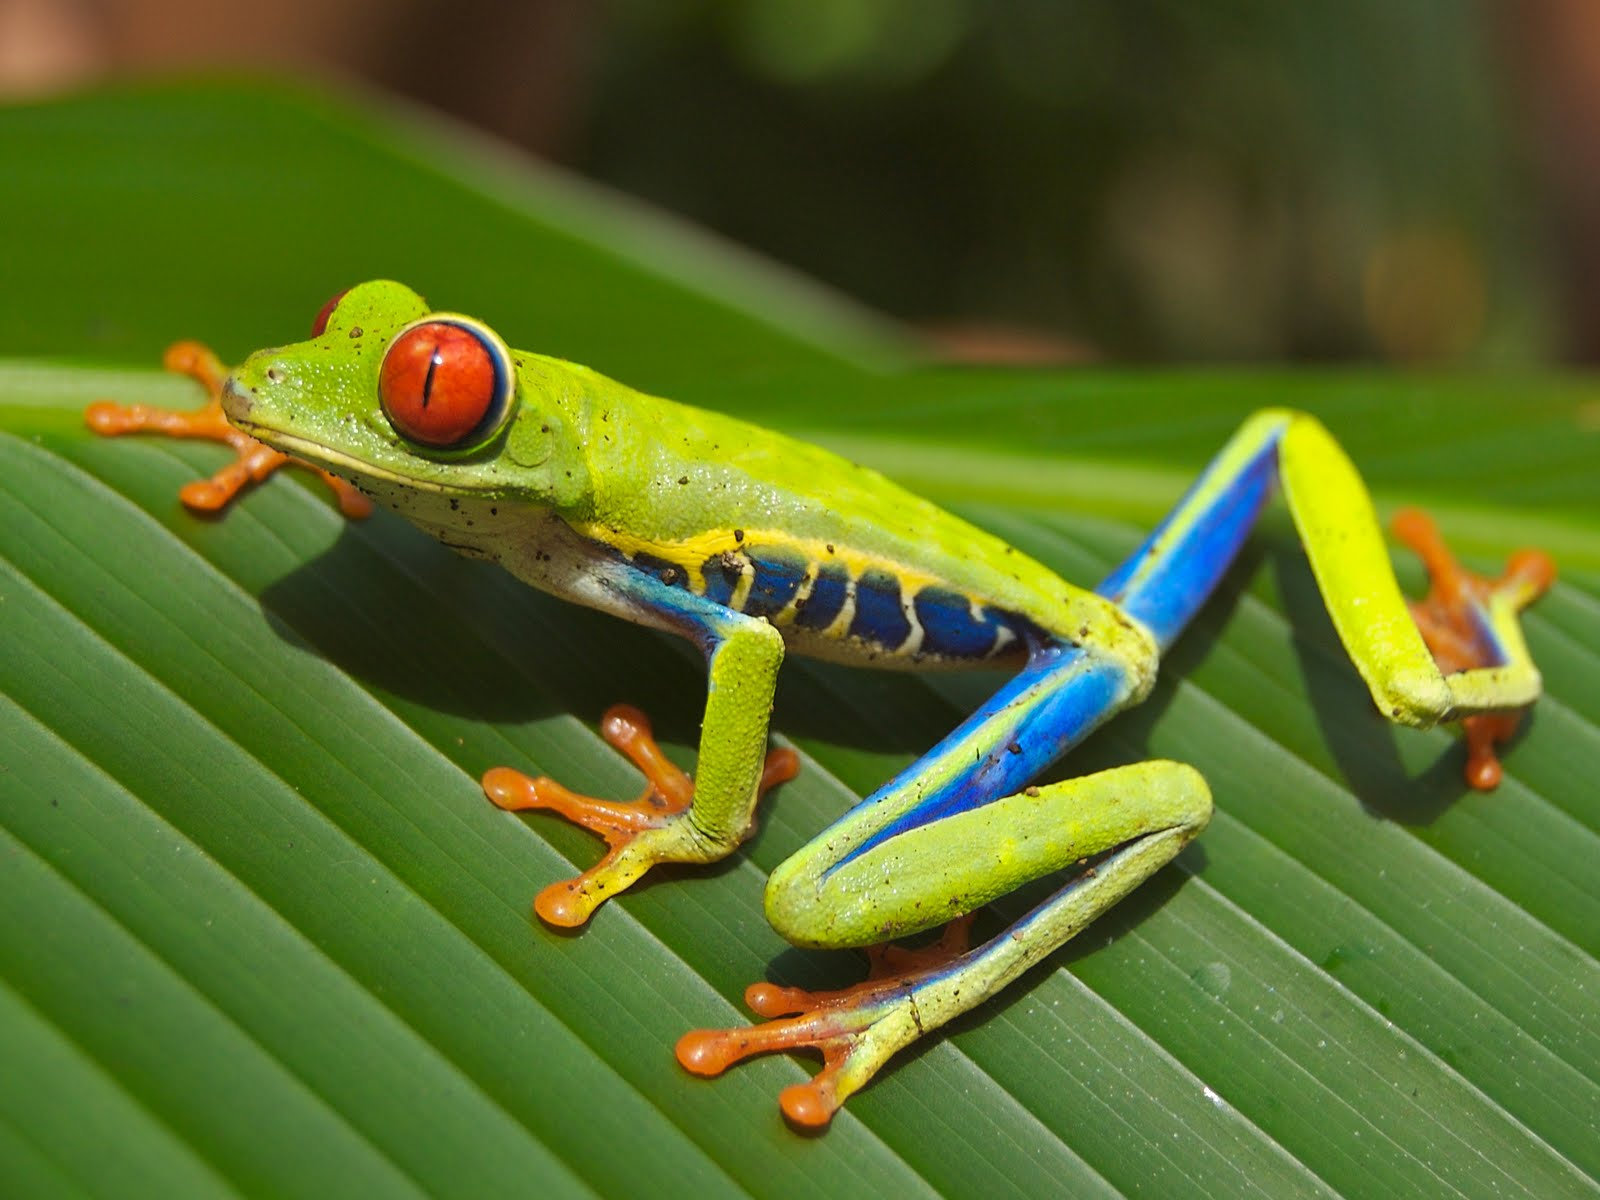
\includegraphics[scale=0.2]{frog.jpg}
		\caption{
			Step 4
		}
		\label{fig:h-adapt-two-grid-4}
	\end{subfigure}
\end{figure}




\chapter{Project documentation} \label{chap:docs}

\newcommand{\uml}[2] {
	\begin{figure}[H]
		\centering
		\caption{#1}
		\begin{mpost}[mpsettings=input metauml;]
			#2
		\end{mpost}
	\end{figure}
}

\bt

\section{Some clever stuff} \label{sec:cuda}

\bt

\section{API components overview} \label{sec:api-overview}

Nice UML no. 1...

\uml{IsogeometricFEM class} {
	Class.C("IsogeometricFEM") ()
		("+ apply(pde: PDE, bcs: BoundaryConditions,
			base: BsplineBase, solver: Solver, femConfig: FEMConfig)");
	drawObject(C);
}

Nice UML no. 2...

\uml{HAdaptiveIsogeometricFEM interface} {
	Interface.I("HAdaptiveIsogeometricFEM")
		("+ apply(pde: PDE, bcs: BoundaryConditions,
			adaptationThreshold: Double, solver: Solver, femConfig: FEMConfig)");
	classStereotypes.I("<<interface>>");
	drawObject(I);
}


\section{Detailed API specification and class diagrams} \label{sec:api-detail}

And another large UML...

\uml{The overall class diagram} {
	Class.IsogeometricFEM("IsogeometricFEM")
		() ("+ apply(...)");

	Class.PDE("PDE")
		("+ lhsCoefs: Function[1..*]", "+ rhs: Function") ();
	IsogeometricFEM.n = PDE.s + (60, -60);

	Class.BoundaryConditions("BoundaryConditions")
		("+ left: Double", "+ right: Double",
		 "+ leftType: BoundaryType", "+ rightType: BoundaryType") ();
	IsogeometricFEM.s = BoundaryConditions.n + (60, 60);

	Interface.Base("Base")
		("+ count(): Int",
		 "+ eval(...): Double",
		 "+ getSupport(no: Int): Range");
	classStereotypes.Base("<<interface>>");
	IsogeometricFEM.w = BsplineBase.e + (-150, 0);

	AbstractClass.GriddedBase("GriddedBase") ()
		("+ getGrid(): PointSequence",
		 "+ getGridSpan(index: Int): IntRange",
		 "+ getSupport(no: Int): Range");
	Base.n = GriddedBase.s + (-80, -60);

	Class.BsplineBase("BsplineBase") ()
		("+ getGrid(): PointSequence",
		 "+ getGridSpan(index: Int): IntRange",
		 "+ getSupport(no: Int): Range");
	Base.n = BsplineBase.s + (80, -60);

	Interface.Solver("Solver")
		("+ apply(...)");
	classStereotypes.Solver("<<interface>>");
	IsogeometricFEM.s = Solver.n + (-60, 60);

	Class.GaussSolver("GaussSolver")
		() ("+ apply(...)");
	Solver.e = GaussSolver.w + (-60, 0);

	Class.MultifrontalSolver("MultifrontalSolver")
		() ("+ apply(...)");
	Solver.s = MultifrontalSolver.n + (0, 60);


	drawObjects(
		IsogeometricFEM,
		PDE, BoundaryConditions,
		Base, GriddedBase, BsplineBase,
		Solver, GaussSolver, MultifrontalSolver
	);

	link(dependency)(IsogeometricFEM.n -- PDE.s);
	link(dependency)(IsogeometricFEM.n -- BsplineBase.s);
	link(dependency)(IsogeometricFEM.s -- BoundaryConditions.n);
	link(dependency)(IsogeometricFEM.s -- Solver.n);
	link(realization)(GriddedBase.s -- Base.n);
	link(realization)(BsplineBase.s -- Base.n);
	link(realization)(GaussSolver.w -- Solver.e);
	link(realization)(MultifrontalSolver.n -- Solver.s);
}



\chapter{Evaluation of the results} \label{chap:evaluation}


\chapter{Conclusions and future works} \label{chap:conclusions}

\section{Achieved goals and observations}

\bt 

\section{Areas for development}

\bt



\cleardoublepage % to ensure that the page reference is correct
\addcontentsline{toc}{chapter}{\listfigurename}
\listoffigures

\begingroup
	\let \clearpage \relax % to suppress page break

	\cleardoublepage
	\addcontentsline{toc}{chapter}{\listalgorithmname}
	\listofalgorithms
\endgroup

\nocite{*} % forces bibtex to include all citations, whether or not they were referred to in the paper

\cleardoublepage
\addcontentsline{toc}{chapter}{Bibliography}
\bibliographystyle{bib-style}
\bibliography{bibliography}

\end{document}

% todo: show bibliography on hover

